Once you have implemented the basics, you can add a Congestion Control Algorithm (CCA) to handle overloading in the network. You will implement TCP Reno, as discussed in class. Hence, the number of outstanding (unACKed) packets will now be be min(window size, congestion window size). You will have to demonstrate to us using traces of real connections that your TCP Reno implementation uses Additive Increase under normal operation, and Multiplicative Decrease under loss.

\subsection{Learning Objectives}
With this section, you will learn how TCP manages to maintain a view of the network state, as well as how the TCP state machine for congestion control works (shown below). Implementing TCP Reno will allow you to transfer data faster as you utilize more available bandwidth for data transmission. Additionally, fast recovery will allow you efficiently recover when packets have been lost. 


\subsection{Checkpoint 2 Tasks}
\begin{enumerate}
    \item Basics - Review and understand the TCP congestion control state machine in depth! \cite{state_machine}
    
    \item 
    Update the your code from Checkpoint 1 to add a new parameter, the congestion window: \texttt{cwnd}. The size of your sending window should now be the minimum of \texttt{cwnd} and the advertised window. You should additionally maintain that the total amount of data buffered for the application (unread data, both ordered and unordered bytes) should be less than \texttt{MAX\_NETWORK\_BUFFER}. 
    
    \item Congestion Control - Implement the slow start and congestion avoidance features of the state machine, this should make your implementation like TCP Tahoe. 
    
    \item Fast Recovery - Implement fast recovery, this should move your implementation from Tahoe to Reno. Note, you only need to implement TCP Reno, not TCP NewReno.
    
    \item Make sure to test your new features with many different network settings using \texttt{tcconfig}. You should transmit a large file again using your TCP implementation, like you did in Checkpoint 1, set the bandwidth small in relation to the size of your file (ex: transferring 100Mb file, 1Mbps bandwidth) and add packet loss (ex: 5\%) in order to see the TCP sawtooth pattern.
\\

\texttt{Here is a copy of the full state machine}\\
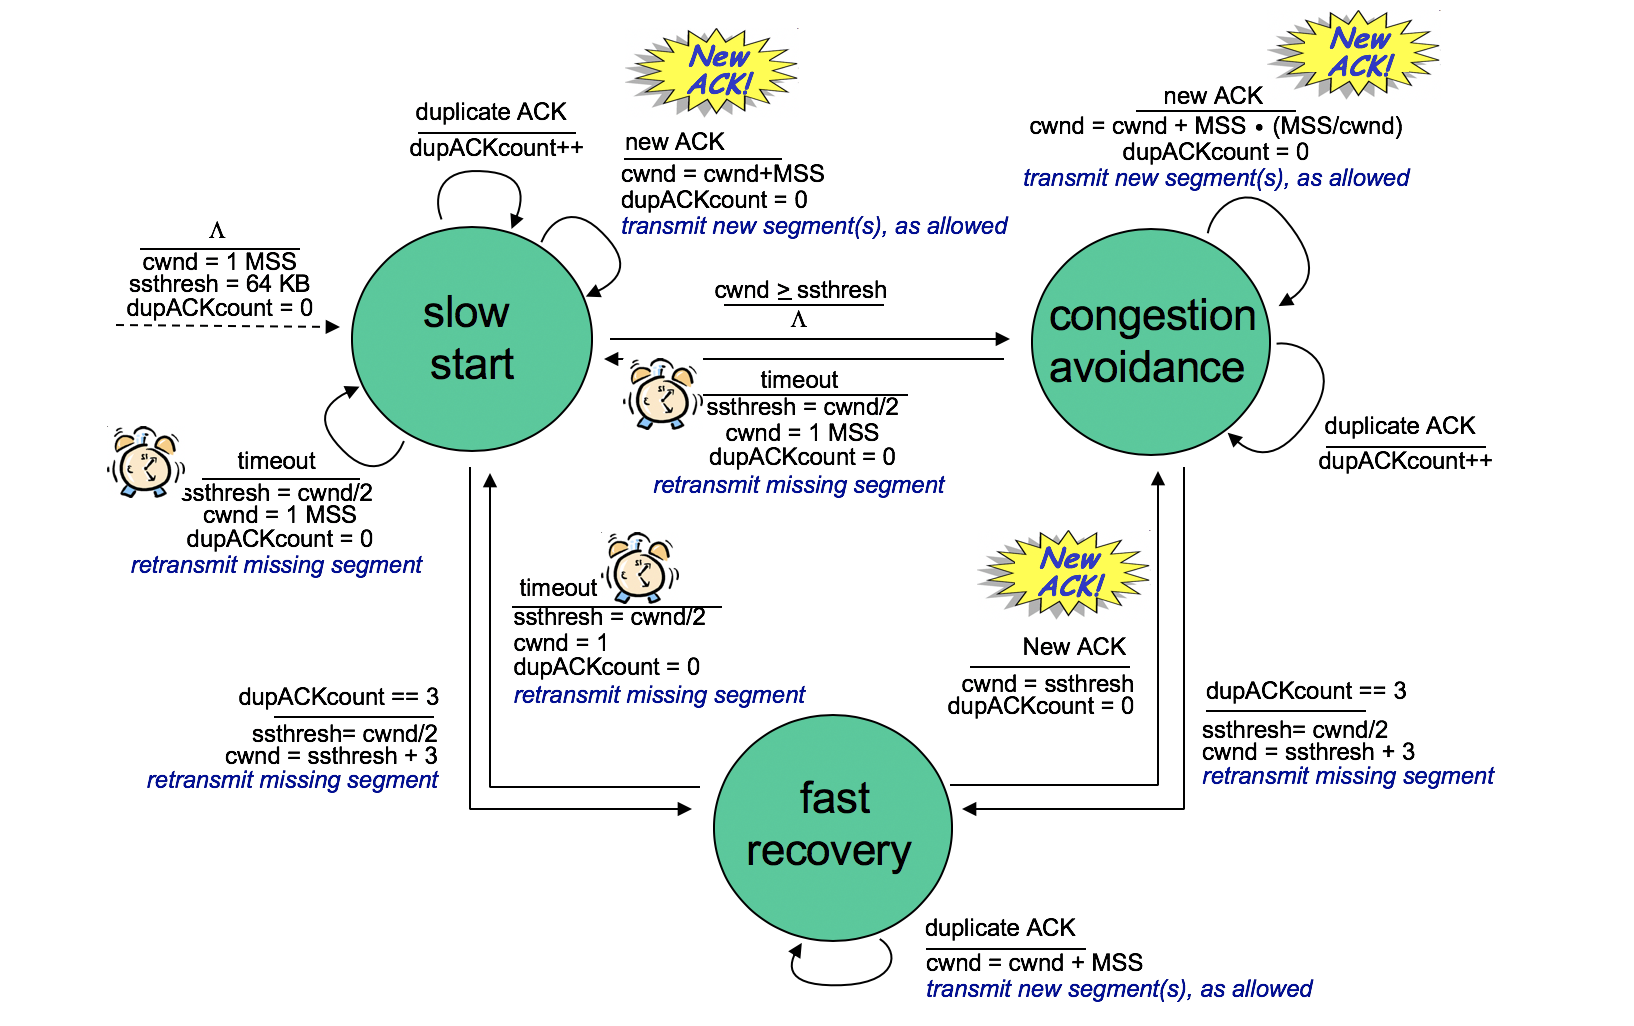
\includegraphics[scale=0.3]{image.png}

\end{enumerate}


Here are the values from \texttt{grading.h} you must use in your code for this checkpoint. We will test your code (and you should too!) by changing these values. All of these values are in bytes.

\begin{enumerate}
    \item \texttt{WINDOW\_INITIAL\_WINDOW\_SIZE}: Initial window size for slow start. In slow start, you should initially set \\ \texttt{cwnd} = \texttt{WINDOW\_INITIAL\_WINDOW\_SIZE}.
    \item \texttt{WINDOW\_INITIAL\_SSTHRESH}: \texttt{ssthresh} value for congestion control. In slow, start, you should initially set \texttt{ssthresh} = \texttt{WINDOW\_INITIAL\_SSTHRESH}.
    \item \texttt{MAX\_LEN}: Max packet length of any packet - including header. This value will not change and will always remain fixed.
    \item \texttt{MAX\_NETWORK\_BUFFER}: Maximum number of bytes that the TCP implementation can hold/buffer for the application. (This includes unread, ordered and unordered bytes received on the network, and received by the application). Thus, the size of your \texttt{sending\_buf} should be set to \texttt{MAX\_NETWORK\_BUFFER} and the size of  \texttt{received\_buf} should be set to \texttt{MAX\_NETWORK\_BUFFER}.
\end{enumerate}


